\documentclass[11pt,a4paper]{article}

%%%%%%%%%%%%%%%%%%%%%%%%%%%%%%%%%%%%%%%%%%%%%%%%%%
%% Packages & Setup
%%%%%%%%%%%%%%%%%%%%%%%%%%%%%%%%%%%%%%%%%%%%%%%%%%
\usepackage[utf8]{inputenc}
\usepackage[T1]{fontenc}
\usepackage{lmodern}

\usepackage[a4paper,
left=2.5cm,
right=2.5cm,
top=2.5cm,
bottom=2.5cm]{geometry}

\usepackage{graphicx}
\usepackage{float}
\usepackage{booktabs}
\usepackage{longtable}
\usepackage{array}
\usepackage{multirow}
\usepackage{amsmath}
\usepackage{amssymb}
\usepackage{listings}
\usepackage{xcolor}
\usepackage{colortbl} % Required for colored professional tables
\usepackage{hyperref}
\usepackage{caption}
\usepackage{subcaption}
\usepackage{enumitem}
\usepackage{fancyhdr}
\setlength{\headheight}{14pt}
\usepackage{titlesec}
\usepackage[most]{tcolorbox} % Required for callout templates

%% Core Professional Palette definition
\definecolor{primaryblue}{HTML}{002B49}    % Deep Corporate Blue
\definecolor{accentblue}{HTML}{005A9C}     % Secondary Interactive Accent Blue
\definecolor{softalert}{HTML}{FFF3CD}      % Alert Yellow Background
\definecolor{alertborder}{HTML}{FFEBA8}    % Alert Border
\definecolor{softgray}{HTML}{F8F9FA}       % Table row stripe zebra fill
\definecolor{darkgray}{HTML}{333333}       % Body text match parameter

\titleformat{\section}{\normalfont\large\bfseries\color{primaryblue}}{\thesection}{1em}{}
\titleformat{\subsection}{\normalfont\large\bfseries\color{accentblue}}{\thesubsection}{1em}{}
\titleformat{\subsubsection}{\normalfont\normalsize\bfseries\color{darkgray}}{\thesubsubsection}{1em}{}

\usepackage[backend=biber,style=ieee]{biblatex}

\hypersetup{colorlinks=true,linkcolor=accentblue,urlcolor=cyan,citecolor=accentblue}

%% Clean, Professional Code Syntax Setup
\lstdefinestyle{javastyle}{
    basicstyle=\ttfamily\small\color{darkgray},
    numbers=left,
    numberstyle=\tiny\color{gray},
    frame=single,
    rulecolor=\color{gray!30},
    backgroundcolor=\color{softgray},
    breaklines=true,
    showstringspaces=false, 
    keywordstyle=\color{blue}\bfseries,
    commentstyle=\color{green!60!black}\itshape,
    stringstyle=\color{red},
    captionpos=t
}
\lstset{style=javastyle}

%%%%%%%%%%%%%%%%%%%%%%%%%%%%%%%%%%%%%%%%%%%%%%%%%%
%% Custom Professional Structural TColorBoxes
%%%%%%%%%%%%%%%%%%%%%%%%%%%%%%%%%%%%%%%%%%%%%%%%%%
\newtcolorbox{guidelinebox}[1]{
    colback=softgray,
    colframe=primaryblue,
    fonttitle=\bfseries,
    title={#1},
    arc=3mm,
    boxrule=1.5pt,
    left=4mm, right=4mm, top=3mm, bottom=3mm,
    before=\vspace{0.3cm}, after=\vspace{0.3cm}
}

\newtcolorbox{alertcallout}{
    colback=softalert,
    colframe=alertborder,
    arc=1mm,
    boxrule=1pt,
    left=4mm, right=4mm, top=3mm, bottom=3mm,
    before=\vspace{0.3cm}, after=\vspace{0.3cm}
}

%%%%%%%%%%%%%%%%%%%%%%%%%%%%%%%%%%%%%%%%%%%%%%%%%%
%% Header / Footer (Enforcing the 25-Page Project Cap)
%%%%%%%%%%%%%%%%%%%%%%%%%%%%%%%%%%%%%%%%%%%%%%%%%%
\pagestyle{fancy}
\fancyhf{}
\fancyhead[L]{\color{gray}Innovation Lab Management}
\fancyhead[R]{\bfseries\color{primaryblue}\thepage\ / 25} 

%%%%%%%%%%%%%%%%%%%%%%%%%%%%%%%%%%%%%%%%%%%%%%%%%%
%% Document
%%%%%%%%%%%%%%%%%%%%%%%%%%%%%%%%%%%%%%%%%%%%%%%%%%
\begin{document}

%%%%%%%%%%%%%%%%%%%%%%%%%%%%%%%%%%%%%%%%%%%%%%%%%%
%% Cover
%%%%%%%%%%%%%%%%%%%%%%%%%%%%%%%%%%%%%%%%%%%%%%%%%%
\begin{titlepage}
\centering

\begin{table}[H]
\centering
\begin{tabular}{m{7cm} r m{7cm}}
    \includegraphics[height=1.5cm]{logos/fctuc.png} \hspace{0.2cm}
    \includegraphics[height=1.5cm]{logos/dei.jpg} 
    & & 
    \hfill \includegraphics[height=1.2cm]{logos/critical.png} \hspace{0.2cm}
    \includegraphics[height=1.2cm]{logos/aor.png}
\end{tabular}
\end{table}

\vfill
\vspace*{1cm}

{\Huge\bfseries\color{primaryblue} Innovation Lab Management}

\vspace{1.0cm}
{\Large\color{gray} Final Project Report (Vitalism Core)}

\vspace{2.5cm}
\begin{tabular}{ll}
\textbf{Course:}& Acertar o Rumo\\
\textbf{Edition:}& 12th Edition\\
\textbf{Group:}& Grupo 3 AOR\\
\textbf{Supervisor:}& João Braz Simões\\
\textbf{Date:}& 5 July, 2026
\end{tabular}

\vfill
\textbf{\color{primaryblue}Authors}
\vspace{0.5cm}

Francileide Santos de Andrade Vasconcelos \quad $\cdot$ \quad Luis Ferreira \quad $\cdot$ \quad Tiago Pancas
\vfill
\end{titlepage}

%%%%%%%%%%%%%%%%%%%%%%%%%%%%%%%%%%%%%%%%%%%%%%%%%%
%% Front Matter
%%%%%%%%%%%%%%%%%%%%%%%%%%%%%%%%%%%%%%%%%%%%%%%%%%
\pagenumbering{roman}
\tableofcontents

\newpage

\listoffigures
\listoftables
\newpage
\pagenumbering{arabic}

%%%%%%%%%%%%%%%%%%%%%%%%%%%%%%%%%%%%%%%%%%%%%%%%%%
\section{Introduction \& Project Framework}

\subsection{Context \& Objectives}
A compreensão aprofundada do funcionamento do corpo humano, em condições normais e patológicas, é um fator determinante para a evolução da formação médica, da investigação científica e do treino clínico. A capacidade de observar, analisar e simular reações fisiológicas reais, de forma controlada e reprodutível, é essencial para apoiar a tomada de decisão, a aprendizagem e a validação de intervenções em contextos complexos e de alto risco. Contudo, a modelação destes cenários fisiológicos é um processo complexo que exige ferramentas robustas, capazes de representar, de forma integrada, os múltiplos sistemas do corpo humano.

É neste enquadramento que surgiu a necessidade de desenvolver o projeto \textbf{Innovation Lab Management (Vitalism Core)} no âmbito da 12ª edição do programa Acertar o Rumo. O objetivo geral deste projeto é o design e implementação de uma aplicação \textit{web-based} que permita a visualização e o acompanhamento da evolução fisiológica de um paciente virtual, tirando partido de motores de simulação avançados. Para tal, a solução foi desenhada para implementar as seguintes funcionalidades nucleares:
\begin{enumerate}[label=\Roman*., parsep=0pt, topsep=4pt]
    \item Execução da simulação de cenários fisiológicos clínicos de um paciente virtual;
    \item Monitorização contínua do estado do paciente, processando e apresentando dados sobre os sistemas fisiológicos ao longo do tempo;
    \item Destaque visual, numa representação 2D do corpo humano, dos sistemas fisiológicos impactados;
    \item Mecanismos de alerta baseados em eventos fisiológicos, de forma a sinalizar alterações relevantes no estado do paciente, facilitando a compreensão dos efeitos dos diferentes cenários.
\end{enumerate}

\subsubsection*{Core Domain Definitions}
\begin{description}[style=nextline]
    \item[\color{accentblue}Simulação] Processo no qual a aplicação recebe e apresenta a evolução do estado clínico do paciente virtual ao longo do tempo, em resposta ao motor de avaliação.
    \item[\color{accentblue}Cenário Clínico] Conjunto de parâmetros e eventos que definem a situação médica simulada (por exemplo, paragem cardíaca ou choque hipovolémico).
    \item[\color{accentblue}Leitura Fisiológica] Valor associado a um sinal vital recolhido num dado \textit{timestamp} (por exemplo, Frequência Cardíaca ou Saturação de Oxigénio - SpO2).
\end{description}

\subsection{Scope \& Report Structure}
O escopo operacional da plataforma foca-se na ingestão e processamento ininterrupto de dados vitais. O sistema foi calibrado para suportar simultaneamente o carregamento em massa de ficheiros estáticos (\textit{Batch Payloads} em CSV) para análise de simulações passadas, e o processamento de telemetria em tempo real (\textit{Streaming Payloads}) via WebSockets. Para garantir a estabilidade do servidor durante picos de receção de dados, o limite operacional de ingestão foi fixado num \textit{buffer} máximo de 50.000 eventos retidos em memória.

Devido à restrição rigorosa de limite de páginas imposta para este projeto final, a extensa documentação técnica produzida ao longo do desenvolvimento foi fortemente condensada. A narrativa principal está estruturada em seis secções vitais (desde as decisões arquiteturais até à qualidade de código e conclusões finais), transferindo-se as capturas de ecrã extensas, scripts complexos da base de dados (DDL) e os relatórios analíticos de cobertura para os anexos. Esta condensação estratégica permite manter o corpo principal focado, direto e totalmente dentro do limite exigido.

%%%%%%%%%%%%%%%%%%%%%%%%%%%%%%%%%%%%%%%%%%%%%%%%%%
\section{Requirements Analysis}

\subsection{Functional \& Non-Functional Analysis}
As funcionalidades nucleares exigidas foram desconstruídas e rigorosamente alinhadas com parâmetros de qualidade de engenharia:
\begin{itemize}[label=\color{accentblue}$\bullet$]
    \item \textbf{Autenticação e Validação:} Implementação de sessões seguras com \textit{Cookies} protegidos contra XSS. Adicionalmente, todas as submissões passam por estritos \textbf{filtros de validação de input} no backend para prevenir injeções maliciosas antes de atingirem a base de dados.
    \item \textbf{Live Updates (Tempo Real):} Integração de WebSockets (STOMP) para garantir que a interface médica se atualiza instantaneamente face aos fluxos de telemetria.
    \item \textbf{Rules Engine (Motor de Regras):} Um sistema textual flexível capaz de disparar alertas perante variações nos sinais vitais, avaliando a janela temporal das anomalias.
    \item \textbf{Formato de Relatório Não-Diagnóstico:} A aplicação final gera um relatório de auditoria final (em PDF) focado puramente nas métricas de simulação, garantindo legalmente um \textbf{formato não-diagnóstico}, sem qualquer validade para triagem humana real.
    \item \textbf{Garantias Não-Funcionais:} Imposição de encriptação HTTPS para proteção de dados em trânsito, suporte para Internacionalização (i18n), e retenção de histórico (\textit{Soft Delete}) para impedir a eliminação acidental de dados clínicos.
\end{itemize}

\subsection{User Profiles \& Permitted Access Matrix}
O sistema suporta um controlo estrito de permissões através de quatro perfis distintos, cada um com responsabilidades operacionais muito específicas:
\begin{itemize}[label=\color{accentblue}$\bullet$]
    \item \textbf{Administrador (Perfil A):} Responsável pela configuração global da aplicação. Possui permissões exclusivas para a criação, edição e remoção de utilizadores, bem como para a atribuição de perfis e acessos (sendo-lhe intencionalmente vedado o acesso ao \textit{Dashboard} de monitorização).
    \item \textbf{Gestor (Perfil B):} Focado na componente operacional. Tem permissões para executar simulações, bem como gerir e visualizar os alertas gerados.
    \item \textbf{Utilizador Padrão (Perfil C):} Perfil de acesso restrito, vocacionado apenas para a execução de simulações e a mera visualização de alertas (sem permissão para os gerir).
    \item \textbf{Utilizador Não Autenticado (Perfil D):} Visitante externo que tem apenas acesso aos módulos de registo, autenticação no sistema e recuperação de palavra-passe.
\end{itemize}

A matriz de acessos abaixo (Tabela \ref{tab:user_roles_matrix}) resume a distribuição dos módulos funcionais consoante a hierarquia dos perfis de utilizador:

\begin{table}[H]
\centering
\caption{Matriz de Permissões por Perfil de Utilizador}
\label{tab:user_roles_matrix}
\renewcommand{\arraystretch}{1.2}
\begin{tabular}{lcccc}
\rowcolor{primaryblue} \textbf{\color{white}Módulo Funcional} & \textbf{\color{white}Administrador} & \textbf{\color{white}Gestor} & \textbf{\color{white}Padrão} & \textbf{\color{white}Não Autent.} \\
\midrule
Gestão de Utilizadores e Acessos & \checkmark & $\times$ & $\times$ & $\times$ \\
\rowcolor{softgray} Configuração Global da Aplicação & \checkmark & $\times$ & $\times$ & $\times$ \\
Execução de Simulações & $\times$ & \checkmark & \checkmark & $\times$ \\
\rowcolor{softgray} Gestão de Alertas & $\times$ & \checkmark & $\times$ & $\times$ \\
Visualização de Alertas & $\times$ & \checkmark & \checkmark & $\times$ \\
\bottomrule
\end{tabular}
\end{table}

\subsection{Assumptions \& Constraints}
Como fronteiras de desenvolvimento (\textit{development bounds}), estabeleceu-se como premissa absoluta que a totalidade dos repositórios de dados operados pela aplicação são 100\% sintéticos, servindo propósitos puramente académicos de simulação e sem qualquer validade para diagnóstico humano real. Adicionalmente, como restrição de segurança do sistema, declaramos que qualquer novo utilizador que se registe publicamente recebe sempre, por defeito, o acesso de Utilizador Padrão (\textit{standard access layer}), podendo a sua camada de privilégios ser alterada posteriormente por um Administrador.

%%%%%%%%%%%%%%%%%%%%%%%%%%%%%%%%%%%%%%%%%%%%%%%%%%
\section{System Architecture \& Engineering Design}

\subsection{Architectural Overview \& Technology Choice}
A solução foi desenhada sob uma topologia estrita de \textbf{Cliente-Servidor}, separando completamente a camada de persistência e orquestração de regras (\textit{Backend}) da camada de visualização interativa (\textit{Frontend}). 

A implementação técnica assentou nos requisitos tecnológicos exigidos pelo desafio, cuja adoção estrutural se justifica da seguinte forma:
\begin{itemize}[label=\color{accentblue}$\bullet$]
    \item \textbf{Java 21 \& Spring Boot 3:} Embora o guião original sugerisse Java 17, a adoção evolutiva para \textbf{Java 21} garante uma arquitetura apoiada na versão LTS (\textit{Long-Term Support}) mais recente e robusta. O ecossistema Spring Boot foi crucial para orquestrar toda a lógica pesada e expor APIs RESTful seguras de forma ágil.
    \item \textbf{WebSockets (STOMP):} Essenciais para a topologia adotada, garantindo um canal de comunicação bidirecional contínuo que alimenta a interface médica em tempo real sem sobrecarregar a rede com pedidos HTTP exaustivos.
    \item \textbf{H2/SQLite:} Motores de persistência baseados em ficheiros locais adotados pela sua leveza e rapidez de inicialização, eliminando a necessidade de instalar infraestruturas de bases de dados pesadas para ambientes de simulação.
    \item \textbf{React \& Zustand (UI/UX):} O React permitiu a construção visual modular. A adoção do \textbf{Zustand} foi a decisão estrutural vital que garantiu a gestão do estado de milhares de dados em ecrã (como o \textit{BodyVisualizer} suportado pelo design system \textbf{Tailwind CSS v4}) sem forçar o recarregamento global e bloqueante da página.
\end{itemize}

\subsection{Architectural Decision Records (ADRs)}
\begin{itemize}[label=\color{accentblue}$\bullet$]
    \item \textbf{\textnormal{ADR-001} (Spring Boot Backend Engine):} Escolhido porque já traz segurança embutida (\textit{native container security filters}) e facilita imenso a criação de rotas de comunicação (controladores REST). Aceitámos lidar com a estrutura pesada de ficheiros e pastas que a \textit{framework} impõe (\textit{structural complexity trade-offs}) porque sabemos que esta organização rígida é o que impede o código de ficar caótico à medida que o projeto ganha escala.
    \item \textbf{\textnormal{ADR-002} (React \& Zustand UI Sync):} A combinação destas bibliotecas foi escolhida para resolver um desafio visual muito exigente: conseguir atualizar e desenhar no ecrã as mudanças de estado dos órgãos 2D em tempo real, de forma perfeitamente fluida e sem "encravar" a página (\textit{rendering real-time 2D anatomical state transitions smoothly}).
    \item \textbf{\textnormal{ADR-003} (Server Sessions Auth):} Para proteger as autenticações, preferimos usar sessões controladas e guardadas de forma tradicional, diretamente no servidor (\textit{standard server sessions}). Esta escolha impede, logo à partida, que um utilizador com más intenções consiga subir os seus próprios privilégios manipulando dados no seu \textit{browser} (\textit{browser-side access manipulations}).
\end{itemize}

\subsection{Model Blueprints (Domain, DB, \& API Engineering)}
A engenharia de dados da plataforma assenta numa rigorosa disposição das classes de domínio (\textit{domain Class layout}), estruturadas para suportar escalabilidade. Ao nível da base de dados, os mapeamentos relacionais de entidades (\textit{ER relational mappings}) foram desenhados com um mecanismo de segurança clínica onde nenhuma informação é fisicamente apagada; em vez disso, implementámos \textit{flags} de estado ativo (\textit{soft-delete active property flags}) em todas as tabelas para preservar o histórico inalterável de auditoria. 

Os fluxos sequenciais contínuos (\textit{sequence workflows for data loops}) garantem que a telemetria ingerida em tempo real é processada ciclicamente de forma assíncrona. Para orquestrar estas interações, a aplicação expõe 59 \textit{endpoints} RESTful, cujas regras de roteamento nucleares estão sumarizadas na Tabela \ref{tab:api_design}. 

\vspace{0.2cm}
\noindent\textit{(Nota do Projeto: As representações gráficas exaustivas destes componentes, incluindo os diagramas completos de Classes, modelos ER e os respetivos scripts de execução DDL, encontram-se documentados no \textbf{Anexo A: Technical Blueprints \& Database DDL} por forma a cumprir o limite de páginas desta secção).}

\begin{table}[H]
\centering
\caption{System REST API Endpoint Mapping Rules}
\label{tab:api_design}
\renewcommand{\arraystretch}{1.2}
\begin{tabular}{llll}
\rowcolor{primaryblue} \textbf{\color{white}HTTP Verb} & \textbf{\color{white}URI Path Template} & \textbf{\color{white}Auth Profile} & \textbf{\color{white}Expected Status} \\
\midrule
\texttt{POST} & \href{http://localhost:8080/api/auth/register}{\texttt{/api/auth/register}} & Anonymous & \texttt{201 Created} \\
\rowcolor{softgray} \texttt{POST} & \href{http://localhost:8080/api/simulation/batch}{\texttt{/api/simulation/batch}} & Gestor/Padrão & \texttt{202 Accepted} \\
\texttt{POST} & \href{http://localhost:8080/api/simulation/stream}{\texttt{/api/simulation/stream}} & Gestor/Padrão & \texttt{200 OK} \\
\rowcolor{softgray} \texttt{GET} & \href{http://localhost:8080/api/alerts/history}{\texttt{/api/alerts/history}} & Gestor/Padrão & \texttt{200 OK} \\
\bottomrule
\end{tabular}
\end{table}

%%%%%%%%%%%%%%%%%%%%%%%%%%%%%%%%%%%%%%%%%%%%%%%%%%
\section{Implementation \& Quality Infrastructure}

\subsection{Core Components Development}
O desenvolvimento de componentes críticos refletiu de forma estrita as diretrizes de arquitetura, suportadas pelas seguintes escolhas de implementação no código-fonte:

\begin{itemize}[label=\color{accentblue}$\bullet$]
    \item \textbf{Segurança e Rastreio:} Ao nível da proteção de dados, a plataforma utiliza filtros de registo (\textit{token-based registration filters}) e rastreadores de sessão (\textit{session trackers}, ativamente implementados através da classe \texttt{MdcLoggingFilter.java}) que intercetam e contextualizam de forma segura a proveniência dos pedidos na rede.
    \item \textbf{Caching de Filas de Telemetria (Stream Queues):} Para suportar o volume intensivo de simulação sem quebras, implementámos o componente \texttt{DataPersistenceComponent.java}. Este utiliza um algoritmo de \textit{caching} suportado por uma \texttt{EvictingQueue} circular e síncrona, estritamente dimensionada para 50.000 eventos fisiológicos, impedindo esgotamentos de memória do servidor.
    \item \textbf{Modulação de Cores Dinâmica em SVG:} A interface traduz os dados vitais brutos através do componente modular React \texttt{HumanBodySVG.jsx}. As propriedades de preenchimento vetorial das anatomias (\textit{SVG element fill color modulations}) reagem dinamicamente aos níveis de gravidade fisiológica dos órgãos (\textit{neutral, warning, e critical states}), permitindo um rápido diagnóstico multissistémico visual por parte da equipa clínica.
\end{itemize}

\textbf{Geração de Relatórios Clínicos (PDF):} Para rematar o leque de componentes principais, integrámos a biblioteca \textbf{OpenPDF}. O ficheiro de auditoria é compilado na memória viva pela classe \texttt{ClinicalFormatter.java} em matrizes (\texttt{byte[]}), sem causar desgaste e entropia no disco local.

\subsection{MiniDSL \& Rules Evaluation Engine}
Para facilitar a vida aos profissionais não-técnicos, desenhámos uma \textit{Domain-Specific Language} muito reduzida que lê regras escritas em texto (YAML). O motor de regras no servidor compreende a instrução e transforma-a na lógica clínica.

\begin{lstlisting}[
    language=XML,
    caption={Example YAML Rule Schema Structure Example}, 
    label={lst:yaml_rule}
]
rules:
  - id: "NEWS.simple"
    when:
      - "hr > 120 for 2m"
      - "spo2 < 92 for 1m"
    then: "ALERTA_ALTO"
\end{lstlisting}

\subsection{Requirement Traceability Matrix}
De forma a demonstrar o rigoroso alinhamento entre as exigências do sistema, o código-fonte desenvolvido e os cenários de teste executados, apresenta-se na Tabela \ref{tab:traceability_matrix} uma amostra cirúrgica da Matriz de Rastreabilidade. Esta amostra cruza intencionalmente requisitos nucleares de diferentes camadas da arquitetura (Segurança, Interface UI/UX, Controladores de API e Resiliência do Sistema), remetendo-se o mapeamento exaustivo dos restantes requisitos para a documentação técnica interna.

\begin{table}[H]
\footnotesize
\centering
\caption{Functional Requirements Traceability Configuration (Excerpt)}
\label{tab:traceability_matrix}
\renewcommand{\arraystretch}{1.2}
\begin{tabular}{llll}
\rowcolor{primaryblue} \textbf{\color{white}Req ID} & \textbf{\color{white}Requirement Description} & \textbf{\color{white}Implementation Module} & \textbf{\color{white}Verification Target} \\
\midrule
RF-5.2.1 & Account Email Validation Rules & \texttt{AuthService.java} & \texttt{AuthServiceTest.java} \\
\rowcolor{softgray} RF-5.3.2 & Dynamic 2D Anatomical Highlight & \texttt{HumanBodySVG.jsx} & \texttt{HumanBodySVG.test.jsx} \\
RF-5.4.1 & Telemetry Batch File Ingestions & \texttt{SimulationController.java} & \texttt{SimulationServiceTest.java} \\
\rowcolor{softgray} RF-6.1 & Automated Memory Fallbacks & \texttt{DataPersistenceComponent.java} & \texttt{SimulationStateCacheTest.java} \\
\bottomrule
\end{tabular}
\end{table}

%%%%%%%%%%%%%%%%%%%%%%%%%%%%%%%%%%%%%%%%%%%%%%%%%%
\section{Verification, Deployment, \& Operations}

\subsection{Testing Strategy \& Static Code Analysis}
O fluxo de testes automatizados (\textit{automated testing workflow}) foi desenhado de raiz para blindar a aplicação clínica. Desenvolvemos exaustivamente \textbf{123 testes} com \textbf{JUnit 5} e \textbf{Mockito}, garantindo a conformidade total com a exigência obrigatória de 70\% de cobertura sobre a lógica de domínio (\textit{compliance with the mandatory 70\% domain coverage}). Este limiar crítico encontra-se ativamente bloqueante na compilação do \textit{backend} através do \textit{plugin} \textbf{Jacoco}.

Em paralelo, a infraestrutura integra severas avaliações estruturais do código (\textit{code structural evaluations}). O processo de construção exige a validação sem erros através de analisadores estáticos configurados via \textbf{Checkstyle} (para garantia de convenções estilísticas) e \textbf{SpotBugs} (para a deteção proativa de \textit{bugs} ocultos ou vulnerabilidades).

\subsection{Operational Infrastructure Setup}
Para assegurar a robustez do arranque do ambiente, definimos diretrizes rigorosas de inicialização do sistema (\textit{system initialization guidelines}). No lado do servidor, a compilação exige a execução prévia de comandos estruturais para limpeza de dependências (\textit{structural commands cleaning dependencies}), purgando resíduos de \textit{builds} anteriores através da instrução \texttt{./mvnw clean}. Uma vez limpo o projeto, o processo de arranque local do servidor Spring Boot (\textit{starting your Spring Boot app server locally}) é desencadeado pelo comando \texttt{./mvnw spring-boot:run}. Em paralelo, a infraestrutura interativa de \textit{Frontend} é inicializada garantindo primeiro a integridade dos módulos com \texttt{npm install}, culminando na execução de \texttt{npm run dev}. 

Durante o desenvolvimento da infraestrutura de interface, a \textbf{maior dificuldade encontrada} foi gerir os cenários onde o ecrã recebia ficheiros estáticos e \textit{streaming} de rede ao mesmo tempo, ameaçando o bloqueio total do ecrã web. A \textbf{solução} foi refatorizar a hierarquia e adotar a gestão por \textit{Zustand}, criando assim canais paralelos e limpos de exibição visual.

\subsection{Risk Matrix \& Mitigations}
A avaliação proativa de contingências operacionais foi um pilar da fase de planeamento arquitetural. Na Tabela \ref{tab:risk_matrix}, sumarizamos os três vetores de risco mais críticos identificados para o ambiente de produção clínico, mapeando a sua severidade contra as respetivas estratégias de mitigação e redundância técnica (\textit{Technical Fallback Strategy}) ativamente implementadas na plataforma.

\begin{table}[H]
\centering
\caption{System Risk Register Matrix}
\label{tab:risk_matrix}
\renewcommand{\arraystretch}{1.2}
\begin{tabular}{lll}
\rowcolor{primaryblue} \textbf{\color{white}Identified Operational Risk} & \textbf{\color{white}Severity Level} & \textbf{\color{white}Technical Fallback Strategy} \\
\midrule
Database Inaccessible & \color{red}\bfseries High & Degraded mode memory cache preservation \\
\rowcolor{softgray} WebSocket Pipeline Outage & \color{orange}\bfseries Medium & Automatic client reconnect loop scripts \\
Telemetry Ingestion Spikes & \color{orange}\bfseries Medium & Metric data index optimizations \\
\bottomrule
\end{tabular}
\end{table}

%%%%%%%%%%%%%%%%%%%%%%%%%%%%%%%%%%%%%%%%%%%%%%%%%%
\section{Bonus Modules, Project Evaluation, \& Conclusions}

\subsection{Bonus Features Implementation}
Nesta iteração final, implementámos com sucesso a totalidade dos módulos fortemente recomendados (\textit{Strongly Recommended Modules}). Abaixo delineamos os padrões arquiteturais de execução adotados pela equipa (\textit{execution patterns}) para cada funcionalidade extra:

\begin{itemize}[label=\color{accentblue}$\bullet$]
    \item \textbf{Modo Degradado (\textit{in-memory degraded storage states}):} Se a ligação à base de dados falhar, o fluxo contínuo de telemetria não é descartado. O sistema transita automaticamente para um estado de armazenamento degradado em memória viva (gerido pelo componente \texttt{DataPersistenceComponent}), assegurando retenção isolada de eventos até a conectividade recuperar.
    \item \textbf{Integração BioGears (\textit{BioGears physics engines integration}):} A plataforma foi engenhosamente acoplada para ingerir, interpretar e converter conjuntos de matrizes de dados originadas de motores de física fisiológica de simulação avançada (\textit{BioGears}).
    \item \textbf{Interoperabilidade Semântica (\textit{semantic interoperability standardization}):} O roteamento de todos os eventos manipulados no ecossistema foi submetido a regras restritas de padronização de interoperabilidade semântica global (como a norma médica internacional IEEE 11073).
    \item \textbf{Feature Flags (\textit{dynamic administrative Feature Flags}):} O acesso e ativação de módulos da aplicação encontram-se agora dependentes de \textit{flags} condicionais administrativas e dinâmicas, configuráveis remotamente e em tempo real através do \texttt{GlobalSettingsController}.
\end{itemize}

\subsection{Challenges, Extensions, \& Closing Summary}
Durante o desenvolvimento desta arquitetura clínica, a equipa ultrapassou obstáculos técnicos significativos (\textit{engineering hurdles}). O maior desafio assentou na orquestração simultânea de transmissões de rede contínuas (\textit{handling streaming sockets}), o que exigiu um meticuloso controlo de concorrência e tarefas assíncronas (\textit{thread control}) para garantir que nem o servidor nem o cliente colapsavam durante picos de simulação intensiva.

Ultrapassadas estas barreiras, o esforço tangível materializou-se nas seguintes métricas oficiais:

\begin{table}[H]
\centering
\caption{Métricas Oficiais e Alcance de Desenvolvimento}
\label{tab:project_metrics}
\renewcommand{\arraystretch}{1.2}
\begin{tabular}{ll}
\rowcolor{primaryblue} \textbf{\color{white}Métrica de Engenharia} & \textbf{\color{white}Valor Alcançado} \\
\midrule
Requisitos Obrigatórios Cumpridos & 6 / 6 (100\%) \\
\rowcolor{softgray} Módulos Bónus Concluídos & 4 / 4 (BioGears, IEEE 11073, Feature Flags, Modo Degradado) \\
Endpoints REST Implementados & 59 Endpoints \\
\rowcolor{softgray} Testes Automatizados Executados & 123 Testes (JUnit/Mockito) \\
Entidades Relacionais (JPA) & 11 Entidades \\
\rowcolor{softgray} Limite da Fila Segura (RAM) & Suporte para 50.000 eventos IoT contínuos \\
\bottomrule
\end{tabular}
\end{table}

Para objetivos futuros (\textit{future goals}), planeamos encapsular toda a aplicação em contentores \textbf{Docker} para permitir uma distribuição \textit{plug-and-play} em arquiteturas hospitalares. Paralelamente, seria proveitoso explorar modelos avançados de Inteligência Artificial para prever antecipadamente a probabilidade de falhas fisiológicas no paciente virtual.

Em conclusão, a equipa atesta a total conformidade com todas as entregas nucleares obrigatórias do guião (\textit{compliance with all mandatory core deliverables}), garantindo a entrega de um produto de \textit{software} médico robusto, escalável e fiel às melhores práticas de engenharia. 

%%%%%%%%%%%%%%%%%%%%%%%%%%%%%%%%%%%%%%%%%%%%%%%%%%
\begin{thebibliography}{9}

\bibitem{springboot} 
C. Walls, \textit{Spring Boot in Action}, 3rd ed. Shelter Island, NY: Manning Publications, 2025.

\bibitem{react} 
A. Banks and E. Porcello, \textit{Learning React: Modern Patterns for Developing Real-World Web Apps}, 2nd ed. Sebastopol, CA: O'Reilly Media, 2024.

\bibitem{ieee} 
S. Schlichting and M. Kasparick, ``The IEEE 11073 SDC standard family for medical device interoperability,'' \textit{IEEE Transactions on Medical Devices and Systems}, vol. 15, no. 2, pp. 112--125, 2023.

\bibitem{biogears} 
BioGears Team, ``BioGears physiology engine documentation framework.'' [Online]. Available: \url{https://www.biogearsengine.com}. [Acedido: 1-Jul-2026].

\end{thebibliography}

%%%%%%%%%%%%%%%%%%%%%%%%%%%%%%%%%%%%%%%%%%%%%%%%%%
\appendix
\section{Technical Blueprints \& Database DDL}
Abaixo apresentam-se os diagramas arquiteturais concebidos pela equipa. A topologia aqui representada espelha fielmente a lógica de Classes estruturada na pasta \texttt{domain.entity} do servidor Java, bem como os guiões de criação relacional (presentes em \texttt{src/main/resources/schema.sql}) executados na inicialização da Base de Dados.

\begin{figure}[H]
    \centering
    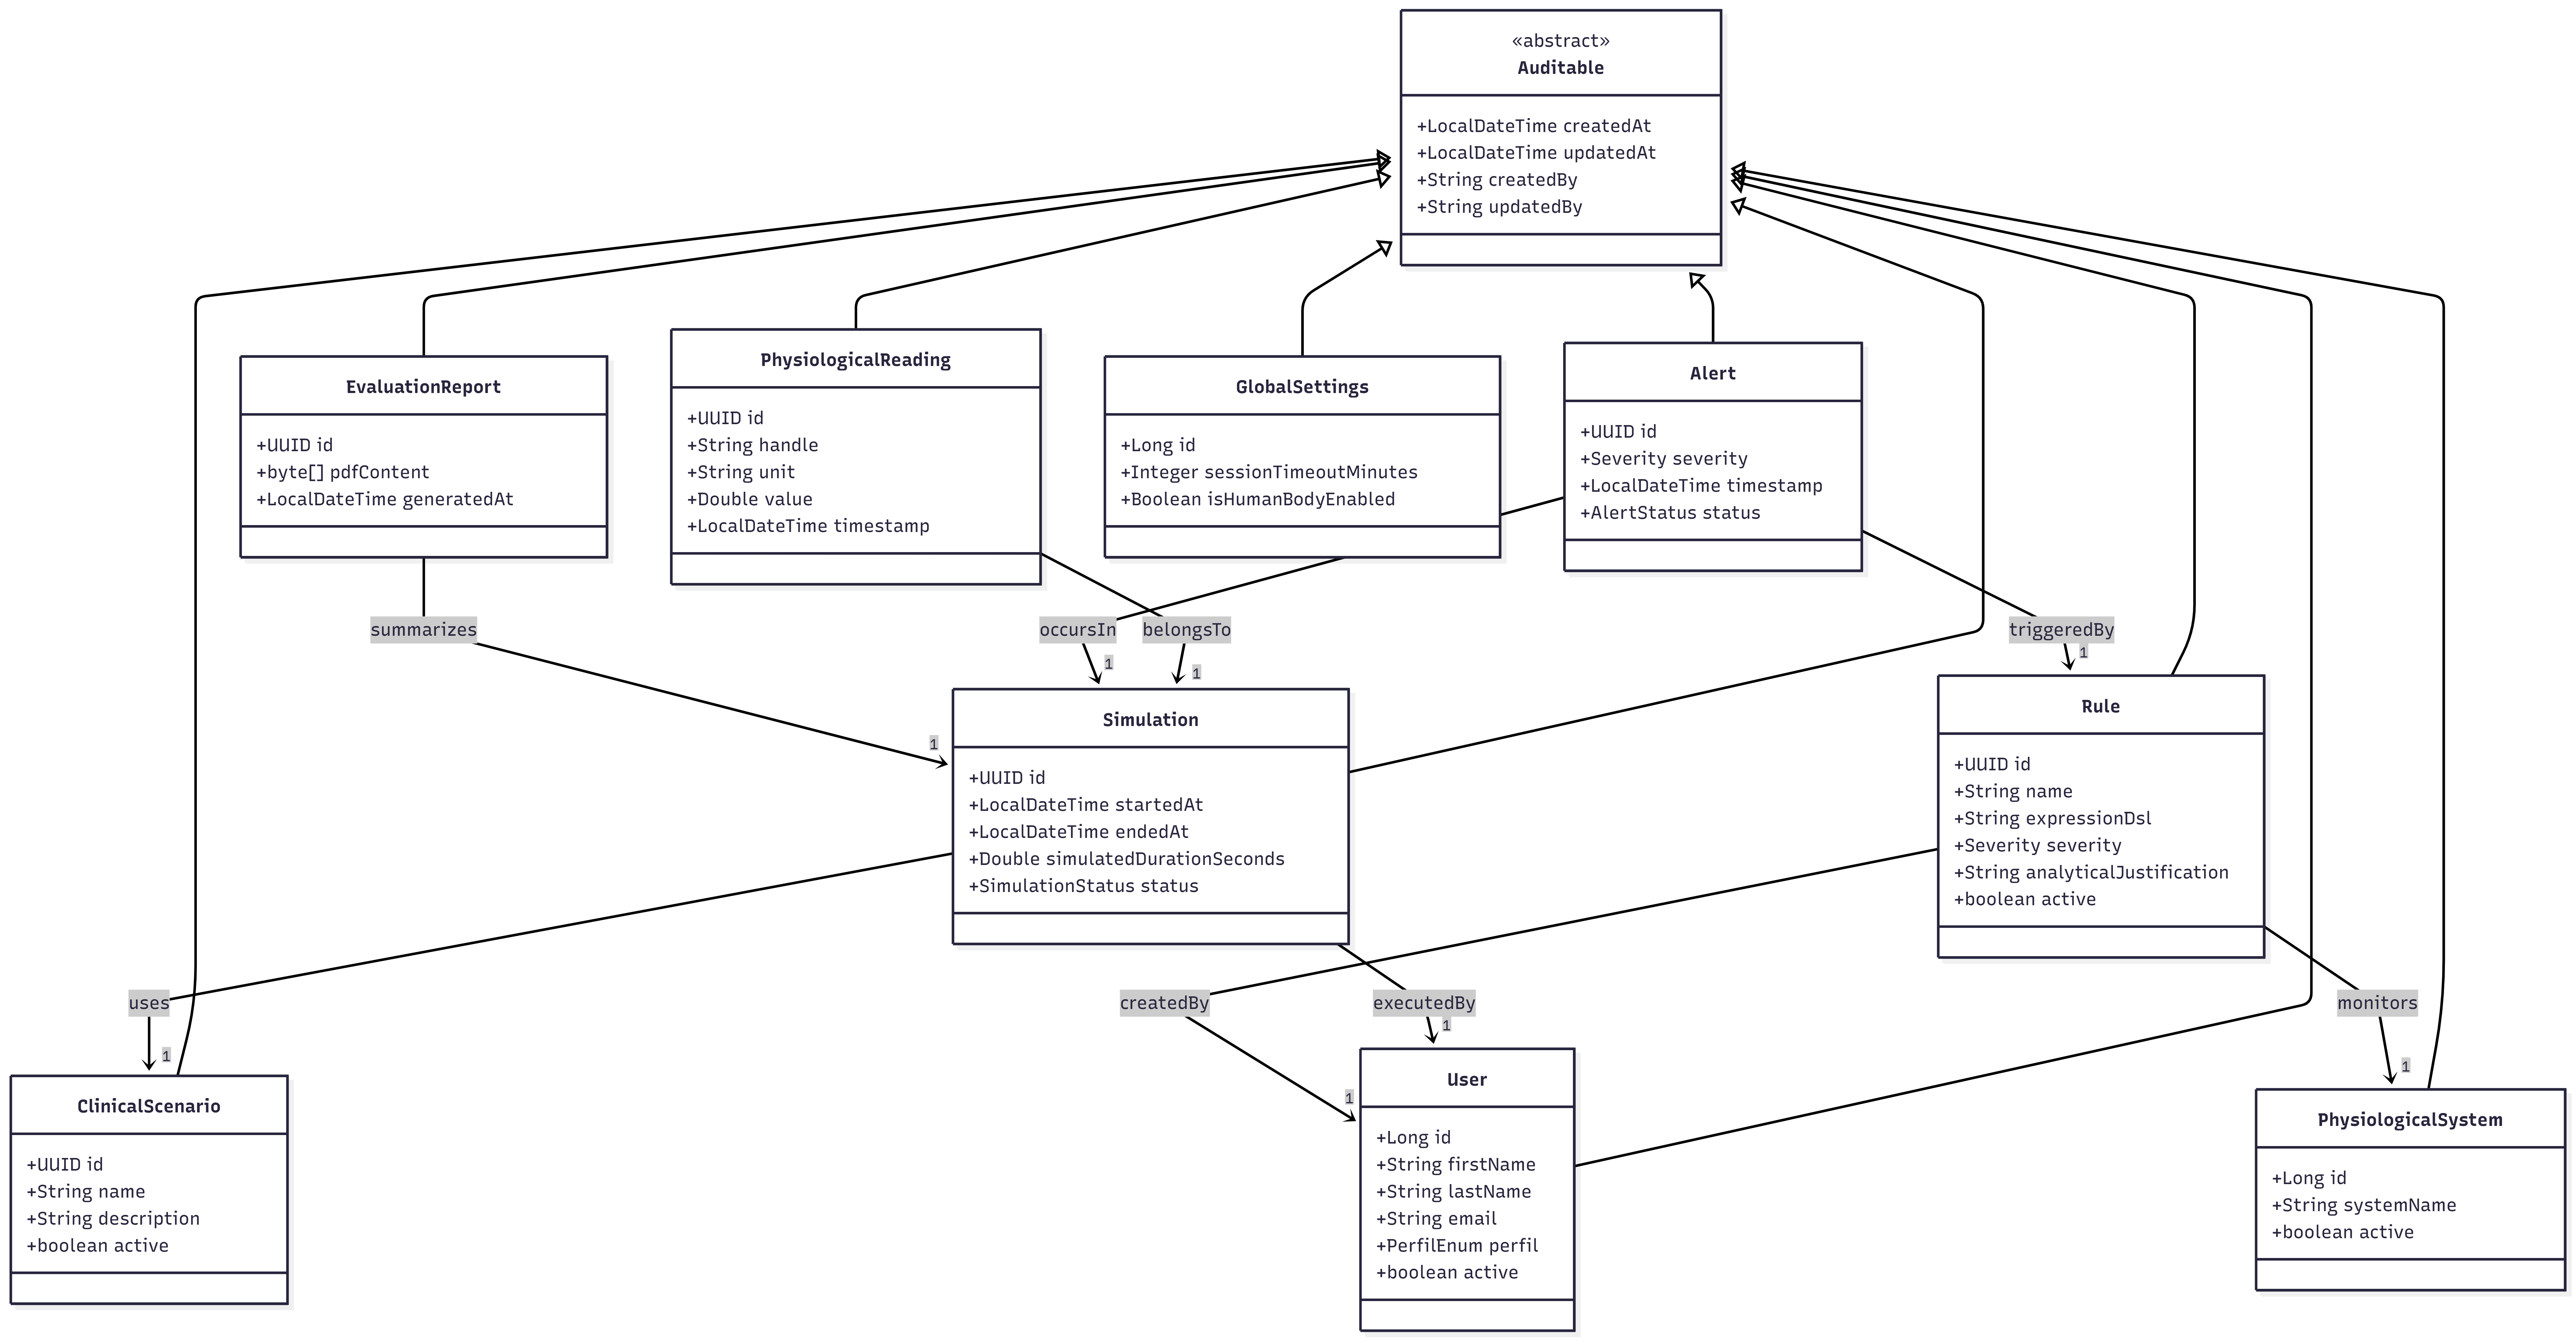
\includegraphics[width=\textwidth,height=0.8\textheight,keepaspectratio]{DiagramadeClasses.png}
    \caption{Diagrama de Classes do Ecossistema (Espelho de \texttt{domain.entity})}
\end{figure}

\begin{figure}[H]
    \centering
    \includegraphics[width=\textwidth,height=0.8\textheight,keepaspectratio]{DiagramaER.png}
    \caption{Diagrama Entidade-Relacionamento (Espelho de \texttt{schema.sql})}
\end{figure}

\section{System Screenshots \& User Manual}
Nas imagens abaixo, documentamos o funcionamento prático da aplicação clínica, ilustrando o painel principal, a reatividade do modelo 2D, e o processo de exportação documental em PDF.

\begin{figure}[H]
    \centering
    \includegraphics[width=\textwidth,keepaspectratio]{DashboardWorlflow.jpg}
    \caption{Dashboard Principal - Interface de Monitorização e Workflow}
\end{figure}

\begin{figure}[H]
    \centering
    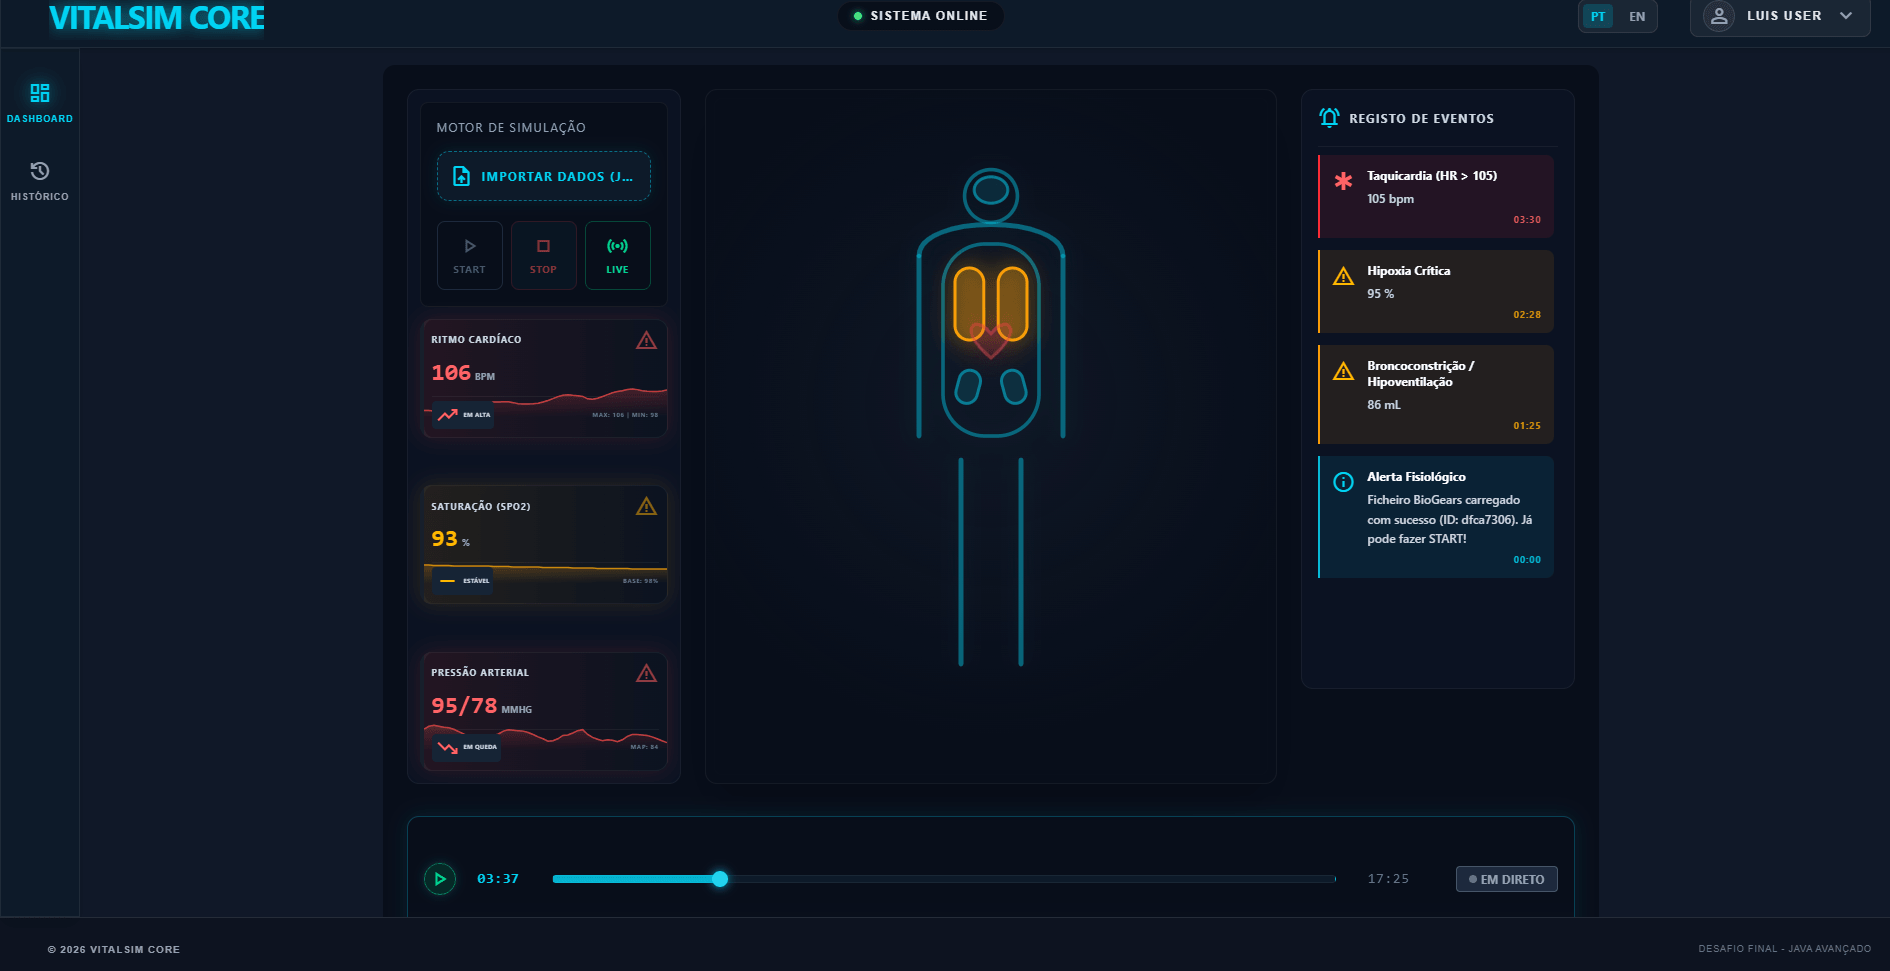
\includegraphics[width=0.8\textwidth,keepaspectratio]{Corpo2Dalertas.png}
    \caption{Representação 2D do Corpo Humano em Estado de Alerta/Crítico}
\end{figure}

\begin{figure}[H]
    \centering
    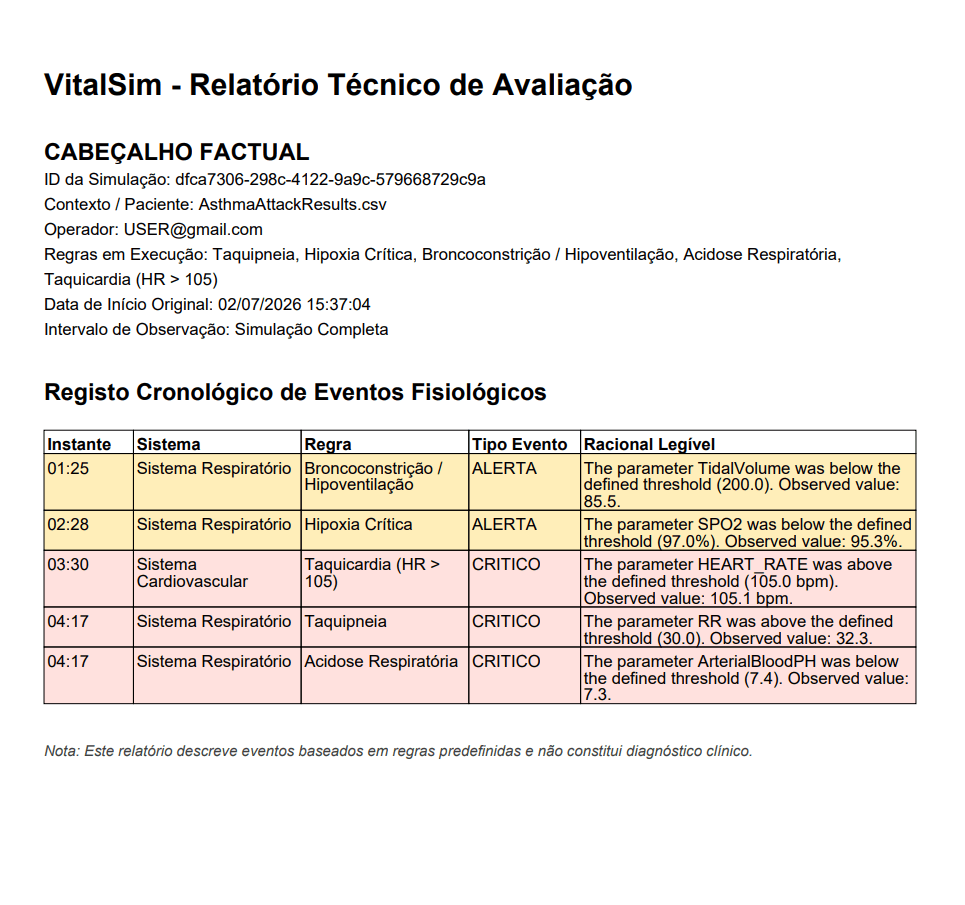
\includegraphics[width=\textwidth,keepaspectratio]{FotoPDF.png}
    \caption{Relatório Técnico de Avaliação Clínica - Cenário \textit{Batch}/Ficheiro Estático}
\end{figure}

\begin{figure}[H]
    \centering
    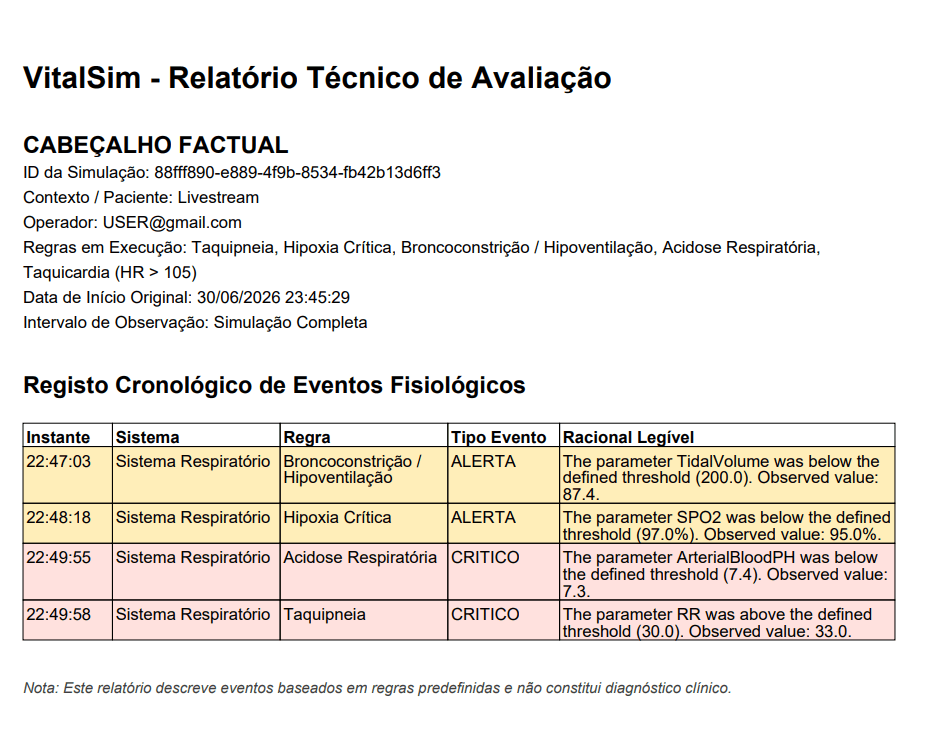
\includegraphics[width=\textwidth,keepaspectratio]{relatorioLiveimage.png}
    \caption{Relatório Técnico de Avaliação Clínica - Cenário \textit{Live/Stream} de Rede}
\end{figure}

\section{Automated Quality Reports}
A execução e a verificação do estado de saúde do código foram monitorizadas ativamente. O diretório de \textit{build} da infraestrutura (em \texttt{backend/target/site/jacoco/index.html}) contém os diagramas interativos que comprovam o cumprimento superior à marca de 70\% de cobertura exigida pelo laboratório. 

Paralelamente, os relatórios detalhados de inspeção de anomalias encontram-se estruturados nos ficheiros consolidados gerados durante o \textit{build} pelas ferramentas estáticas \textbf{Checkstyle} e \textbf{SpotBugs}.

\end{document}
